\documentclass[letterpaper,12pt]{article}\usepackage[]{graphicx}\usepackage[]{color}
%% maxwidth is the original width if it is less than linewidth
%% otherwise use linewidth (to make sure the graphics do not exceed the margin)
\makeatletter
\def\maxwidth{ %
  \ifdim\Gin@nat@width>\linewidth
    \linewidth
  \else
    \Gin@nat@width
  \fi
}
\makeatother

\definecolor{fgcolor}{rgb}{0.345, 0.345, 0.345}
\newcommand{\hlnum}[1]{\textcolor[rgb]{0.686,0.059,0.569}{#1}}%
\newcommand{\hlstr}[1]{\textcolor[rgb]{0.192,0.494,0.8}{#1}}%
\newcommand{\hlcom}[1]{\textcolor[rgb]{0.678,0.584,0.686}{\textit{#1}}}%
\newcommand{\hlopt}[1]{\textcolor[rgb]{0,0,0}{#1}}%
\newcommand{\hlstd}[1]{\textcolor[rgb]{0.345,0.345,0.345}{#1}}%
\newcommand{\hlkwa}[1]{\textcolor[rgb]{0.161,0.373,0.58}{\textbf{#1}}}%
\newcommand{\hlkwb}[1]{\textcolor[rgb]{0.69,0.353,0.396}{#1}}%
\newcommand{\hlkwc}[1]{\textcolor[rgb]{0.333,0.667,0.333}{#1}}%
\newcommand{\hlkwd}[1]{\textcolor[rgb]{0.737,0.353,0.396}{\textbf{#1}}}%

\usepackage{framed}
\makeatletter
\newenvironment{kframe}{%
 \def\at@end@of@kframe{}%
 \ifinner\ifhmode%
  \def\at@end@of@kframe{\end{minipage}}%
  \begin{minipage}{\columnwidth}%
 \fi\fi%
 \def\FrameCommand##1{\hskip\@totalleftmargin \hskip-\fboxsep
 \colorbox{shadecolor}{##1}\hskip-\fboxsep
     % There is no \\@totalrightmargin, so:
     \hskip-\linewidth \hskip-\@totalleftmargin \hskip\columnwidth}%
 \MakeFramed {\advance\hsize-\width
   \@totalleftmargin\z@ \linewidth\hsize
   \@setminipage}}%
 {\par\unskip\endMakeFramed%
 \at@end@of@kframe}
\makeatother

\definecolor{shadecolor}{rgb}{.97, .97, .97}
\definecolor{messagecolor}{rgb}{0, 0, 0}
\definecolor{warningcolor}{rgb}{1, 0, 1}
\definecolor{errorcolor}{rgb}{1, 0, 0}
\newenvironment{knitrout}{}{} % an empty environment to be redefined in TeX

\usepackage{alltt}
\usepackage[top=1in,bottom=1in,left=1in,right=1in]{geometry}
\usepackage{setspace}
\usepackage[colorlinks=true,urlcolor=blue,citecolor=blue,linkcolor=blue]{hyperref}
\usepackage{indentfirst}
\usepackage{multirow}
\usepackage{booktabs}
\usepackage[final]{animate}
\usepackage{graphicx}
\usepackage{verbatim}
\usepackage{rotating}
\usepackage{tabularx}
\usepackage{array}
\usepackage{subfig} 
\usepackage[noae]{Sweave}
\usepackage{cleveref}
\usepackage[figureposition=bottom]{caption}
\usepackage{paralist}
\usepackage{acronym}
\usepackage{outlines}
\usepackage{pdflscape}

% knitr options




\IfFileExists{upquote.sty}{\usepackage{upquote}}{}
\begin{document}

My comments/interpretations:
\begin{itemize}
\item \Cref{fig:tsplot} - time series plot of variables at Bangs Lake.  Nothing too surprising here, but there are noticeable changes in salinity/pH with each event.  Let me know if you like the format, want to add/remove any variables, etc.  
\item \Cref{fig:tukey} - multiple comparison bar plots by event.  These are the same as before, but for Bangs Lake only.  Do we want to include all of these variables?
\item \Cref{fig:phvsal1} - ph v salinity - daily averages of observations grouped by event/stations.  I'm not seeing anything too striking here, at least not like what Jane had in her powerpoint.  My interpretation of her slides was that BL had a different relationship of ph v salinity with increasing freshwater, such that ph stayed high with an inflow event whereas other stations showed the typical positive relationship between ph and salintiy as was observed during `normal conditions'.  I'm not seeing any of that here.
\item \Cref{fig:phvsal2} - ph v salinity - 15 minute observations for different time slices.  This was my attempt at isolating the expected pattern that Jane saw, using different time step aggregations centered on our event categories. My hope was that BL would show the high ph/no relationship with salinity trend for the E1A/E2A plots, whereas the `standard' ph/salinity relationship would be observed in the non-impact year (the year was chosen arbitrarily).  I'm not seeing any of these things so I'm open to suggestions about how to deal with these plots.  It may be worth just showing the time slices Jane had in powerpoint - or show nothing at all.
\item \Cref{tab:ccfwq} - cross-correlation analysis for wq variables - the key to interpreting these tables is the order of the pairwise comparisons on the left and the sign of the lag.  For example, the +40 lag for BC-PC means that the highest correlation between the salinity time series was observed when BC was 40 time steps \emph{behind} PC.  In other words, salinity was positively correlated between the sites and was higher first at PC.  This makes sense based on the locations of the sites.  I think what's interesting is the difference in maximum lags for salinity between the two events - much longer lags for the second event probably related to tidal surge from the storm.  For pH, I don't have too much faith in these differences.  A maximum lag of 1 is just 30 minutes so it could just be related to water movement from normal tidal changes.  I'm not really sure.
\item \Cref{tab:ccfnut} - cross-correlation analysis for nuts.  We may want to reduce some of the variables in this table just for simplicity.  These are harder to interpret than the previous table because there are more variables.  Also note the difference in time scale - here one lag is one month.  I'm not entirely sure how to interpet these results as some make sense and some do not.  For example, a negative max lag for phosphate from BL to PC during the first event makes sense - phosphate was higher first at Bangs Lake.  But why a similar max lag for BC to PC?  This suggests phosphorus was higher first at BC.  It's possible that some of these are just statistical artifacts so we may want to discuss which to include/remove.  
\item \Cref{fig:ordplo} - ordination biplots of nutrient varibles between stations/events.  I'm kind of on the fence with including these plots.  There are some interesting groupings between the sites/events but it's not very distinct.  Here's what I see - First, phosphate shows a strong relationship with BL, particularly during the first event.  Second, there is a lot of overlap between the stations during the non-impact years which is expected.  Third, BC is doing some weird stuff during the second event - it shows a strong relationship to the ammonium - chlorophyll gradient that we don't see in the other sites.  There are probably some other interesting patterns in these plots but that's all I see at first glance.  We should discuss if we want to include these or evaluate in some other way.  
\end{itemize}

\begin{landscape}
\centering\vspace*{\fill}
\begin{figure}[!ht]

{\centering 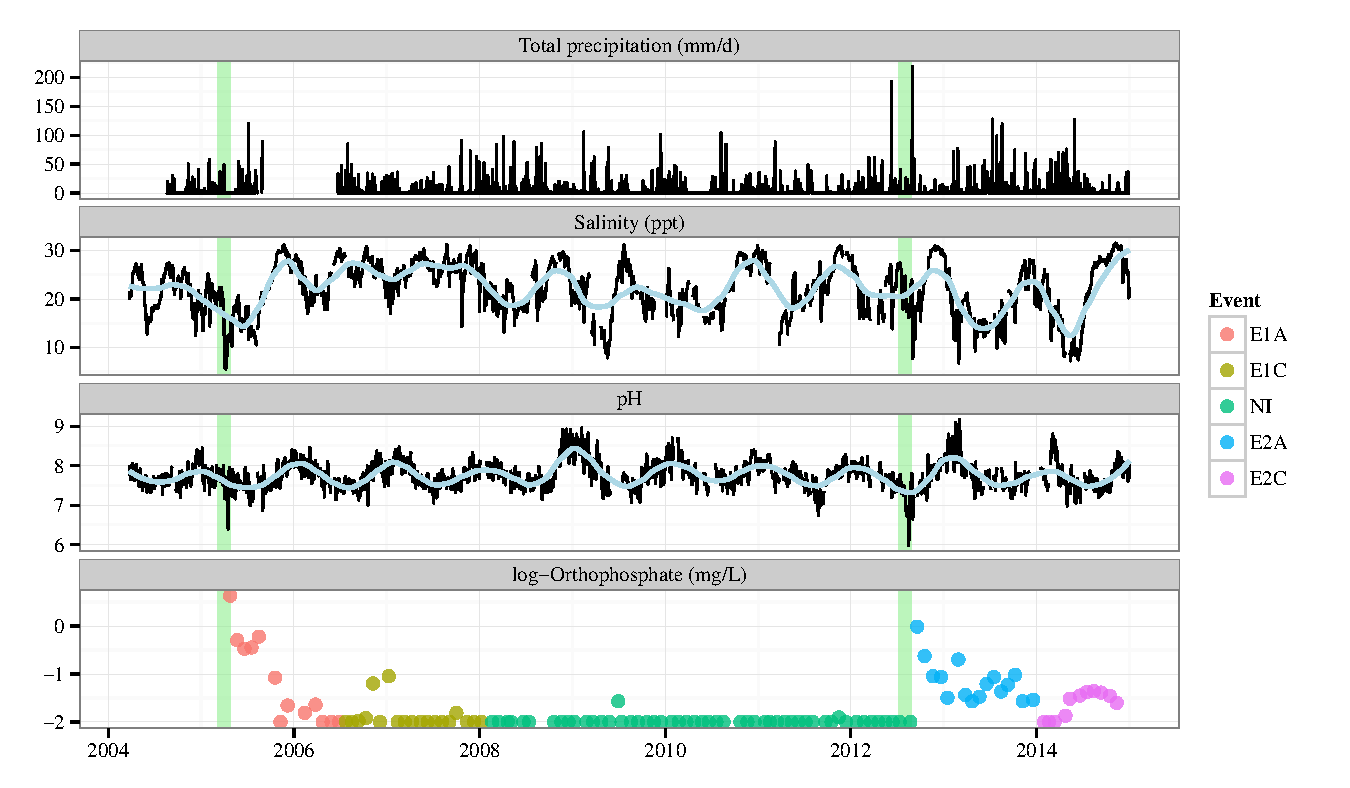
\includegraphics[width=\maxwidth,height=5in]{figs/tsplot-1} 

}

\caption[Time series of total precipitation, salinity, pH, and phosphate for Bangs Lake, Grand Bay reserve]{Time series of total precipitation, salinity, pH, and phosphate for Bangs Lake, Grand Bay reserve.  Vertical green bars indicate a heavy rain event in April 2005 and hurricane Isaac in August 2012.  Salinity and pH include a loess smooth to reduce variability. Orthophosphate is colored by event categories in relation to the vertical green bars.  E1A: event 1 acute, E1C: event 1 chronic, NI: non-impact, E2A: event 2 acute, E2C: event 2 chronic.}\label{fig:tsplot}
\end{figure}


\end{landscape}
\clearpage

\begin{figure}[!ht]

{\centering \includegraphics[width=\maxwidth]{figs/tukey-1} 

}

\caption[Boxplot summaries of nutrient data at Bangs Lake, Grand Bay grouped by events]{Boxplot summaries of nutrient data at Bangs Lake, Grand Bay grouped by events.  Letters indicate events for each nutrient with significantly different observations based on Tukey multiple comparison analysis.  Boxes represent the interquartile range (IQR, 25\textsuperscript{th} to 75\textsuperscript{th} percentile) with the median as the middle horizonal line.  Outliers are present beyond whiskers (1.5$\cdot$IQR). E1A: event 1 acute, E1C: event 1 chronic, NI: non-impact, E2A: event 2 acute, E2C: event 2 chronic.}\label{fig:tukey}
\end{figure}


\clearpage

\begin{figure}[!ht]

{\centering \includegraphics[width=\maxwidth]{figs/phvsal1-1} 

}

\caption[Scatterplots of pH versus salinity for each of the time frames, grouped by station]{Scatterplots of pH versus salinity for each of the time frames, grouped by station.  Observations are daily averages from the continuous time series. E1A: event 1 acute, E1C: event 1 chronic, NI: non-impact, E2A: event 2 acute, E2C: event 2 chronic.}\label{fig:phvsal1}
\end{figure}


\clearpage

\begin{figure}[!ht]

{\centering \includegraphics[width=\maxwidth]{figs/phvsal2-1} 

}

\caption[Scatterplots of pH versus salinity for one month following the two acute exposure events (E1A, E2A) and 2010 during the non-impact (NI) time frame]{Scatterplots of pH versus salinity for one month following the two acute exposure events (E1A, E2A) and 2010 during the non-impact (NI) time frame.  Values are thirty-minute observations at each station. E1A: event 1 acute, NI: non-impact, E2A: event 2 acute.}\label{fig:phvsal2}
\end{figure}


\clearpage

%latex.default(totab, file = "", rowlabel = "Site comparisons",     caption = cap.val, caption.loc = "top", rgroup = rgroups,     n.rgroup = rep(3, 2), cgroup = c("First acute event (E1A)",         "Second acute event (E2A)"), n.cgroup = c(2, 2), rowname = wqres$L1,     label = "tab:ccfwq", insert.bottom = foot.val, col.just = c("r",         "c", "r", "c"))%
\begin{table}[!tbp]
\caption{Results of cross-correlation analyses comparing water quality time series between sites at Grand Bay during the two acute event periods.  Values for pH and salinity (ppt) are the lags in the compared time series between sites at which the maximum correlation was observed.  Negative lags indicate observations were leading at the first site relative to the second, whereas positive lags indicate observations lagged at the first site relative to the second.  One lag is thirty minutes.\label{tab:ccfwq}} 
\begin{center}
\begin{tabular}{lrccrc}
\hline\hline
\multicolumn{1}{l}{\bfseries Site comparisons}&\multicolumn{2}{c}{\bfseries First acute event (E1A)}&\multicolumn{1}{c}{\bfseries }&\multicolumn{2}{c}{\bfseries Second acute event (E2A)}\tabularnewline
\cline{2-3} \cline{5-6}
\multicolumn{1}{l}{}&\multicolumn{1}{c}{Lag}&\multicolumn{1}{c}{Correlation}&\multicolumn{1}{c}{}&\multicolumn{1}{c}{Lag}&\multicolumn{1}{c}{Correlation}\tabularnewline
\hline
{\bfseries pH}&&&&&\tabularnewline
~~BC - PC&$ 1$&$0.25$&&$ 1$&$0.40$\tabularnewline
~~BL - BC&$-1$&$0.58$&&$ 0$&$0.54$\tabularnewline
~~BL - PC&$ 0$&$0.57$&&$ 1$&$0.54$\tabularnewline
\hline
{\bfseries Salinity}&&&&&\tabularnewline
~~BC - PC&$ 1$&$0.47$&&$40$&$0.70$\tabularnewline
~~BL - BC&$ 0$&$0.86$&&$ 0$&$0.92$\tabularnewline
~~BL - PC&$ 5$&$0.73$&&$40$&$0.87$\tabularnewline
\hline
\end{tabular}\end{center}

\footnotesize BC: Bayou Cumbest, BL: Bangs Lake, PC: Point aux Chenes\end{table}

\clearpage

%latex.default(totab, file = "", rowlabel = "Site comparisons",     caption = cap.val, caption.loc = "top", rgroup = rgroups,     n.rgroup = rep(3, 4), cgroup = c("First acute event (E1A)",         "Second acute event (E2A)"), n.cgroup = rep(2, 2), rowname = nutres$L1,     label = "tab:ccfnut", insert.bottom = foot.val, col.just = c("r",         "c", "r", "c"))%
\begin{table}[!tbp]
\caption{Results of cross-correlation analyses comparing nutrient time series between sites at Grand Bay during the two acute event periods.  Values are the lags for each nutrient varialbe in the compared time series between sites at which the maximum correlation was observed.  Negative lags indicate observations were leading at the first site relative to the second, whereas positive lags indicate observations lagged at the first site relative to the second.  One lag is one month.\label{tab:ccfnut}} 
\begin{center}
\begin{tabular}{lrccrc}
\hline\hline
\multicolumn{1}{l}{\bfseries Site comparisons}&\multicolumn{2}{c}{\bfseries First acute event (E1A)}&\multicolumn{1}{c}{\bfseries }&\multicolumn{2}{c}{\bfseries Second acute event (E2A)}\tabularnewline
\cline{2-3} \cline{5-6}
\multicolumn{1}{l}{}&\multicolumn{1}{c}{Lag}&\multicolumn{1}{c}{Correlation}&\multicolumn{1}{c}{}&\multicolumn{1}{c}{Lag}&\multicolumn{1}{c}{Correlation}\tabularnewline
\hline
{\bfseries Chlorophyll a}&&&&&\tabularnewline
~~BC - PC&$ 0$&$0.63$&&$-1$&$0.52$\tabularnewline
~~BL - BC&$ 0$&$0.49$&&$ 1$&$0.49$\tabularnewline
~~BL - PC&$ 0$&$0.92$&&$ 0$&$0.87$\tabularnewline
\hline
{\bfseries Ammonium}&&&&&\tabularnewline
~~BC - PC&$ 0$&$0.99$&&$-4$&$0.38$\tabularnewline
~~BL - BC&$ 0$&$0.96$&&$ 2$&$0.57$\tabularnewline
~~BL - PC&$ 0$&$0.89$&&$ 0$&$0.71$\tabularnewline
\hline
{\bfseries Nitrite + Nitrate}&&&&&\tabularnewline
~~BC - PC&$ 0$&$0.70$&&$ 6$&$0.94$\tabularnewline
~~BL - BC&$ 0$&$0.81$&&$ 0$&$0.11$\tabularnewline
~~BL - PC&$-3$&$0.55$&&$-5$&$0.98$\tabularnewline
\hline
{\bfseries Orthophosphate}&&&&&\tabularnewline
~~BC - PC&$-6$&$0.60$&&$ 1$&$0.78$\tabularnewline
~~BL - BC&$ 0$&$0.62$&&$-1$&$0.79$\tabularnewline
~~BL - PC&$-6$&$0.49$&&$ 0$&$0.82$\tabularnewline
\hline
\end{tabular}\end{center}

\footnotesize BC: Bayou Cumbest, BL: Bangs Lake, PC: Point aux Chenes\end{table}

\clearpage



\begin{landscape}
\begin{figure}
\centering\vspace*{\fill}
\includegraphics[width = 1.3\textwidth]{figs/ordres.pdf}
\caption{Ordination axes from non-metric multidimensional scaling of monthly nutrient observations at each station.  Plots are grouped by events as shown in \cref{fig:tsplot}.  Ellipses around each station represent 95\% confidence intervals for the bivariate distribution of scores between each axis. Stress values measure the departure from monotonicity of the reduced variables in ordination space, with smaller values indicating better fit.  E1A: event 1 acute, E1C: event 1 chronic, NI: non-impact, E2A: event 2 acute, E2C: event 2 chronic.}
\label{fig:ordplo}
\end{figure}
\end{landscape}
\clearpage

\end{document}
